%%This is a very basic article template.
%%There is just one section and two subsections.
\documentclass{thesis}

\usepackage[hidelinks=true]{hyperref}
\usepackage{makeidx}
\usepackage[T1]{fontenc} 
\usepackage[ngerman]{babel}
\usepackage[utf8]{inputenc}
\nonfrenchspacing
\usepackage{url}
\usepackage{breakcites}
\usepackage{epsfig} 
\usepackage{booktabs}
\usepackage{listings}
\usepackage[usenames,dvipsnames,table]{xcolor}
\definecolor{SourceGrau}{gray}{0.98}
\definecolor{lightblue}{rgb}{0.71,0.85,0.96}
\definecolor{dkgreen}{rgb}{0,0.6,0}
\definecolor{gray}{rgb}{0.5,0.5,0.5}
\definecolor{dkgray}{rgb}{0.3,0.3,0.3}
\definecolor{red}{rgb}{0.9,0.0,0.0}
\definecolor{lightgrey}{rgb}{0.7,0.7,0.85}
\definecolor{mauve}{rgb}{0.58,0,0.82}
\lstset{
	basicstyle=\small\ttfamily,						% kleine Schrift, Typewriter
	numbers=left,									% Zeilennummern auf der linken Seite
	tabsize=2,										% Tabs brauchen 2 Leerzeichen
	numberstyle=\tiny,								% Zeilennummern sind winzig
	frame=single,									% einfacher Rahmen um den Code
	aboveskip=1em,									% Abstand zwischen Code(rahmen) und dem Text darüber
	breaklines=true,								% überlange Zeilen werden umgebrochen
	breakautoindent=true, 							% Bei Zeilenumbruch einrücken
	breakindent=2em,
	lineskip=-0.1em,  								% definiert den Zeilenabstand
	showstringspaces=false,							% keine Leerzeichen in Strings anzeigen
	extendedchars=true, 							% Erweiterte Symbole
	keywordstyle=\color{mauve}\bfseries,			% ein bischen bunt kann nicht schaden
	commentstyle=\color{dkgreen}, 
	stringstyle=\color{blue},
  backgroundcolor=\color{SourceGrau},
  columns=flexible,									% Zeichen stehen enger beieinander
  xleftmargin=0.95cm,								% Rand nach links
  xrightmargin=0.75cm,								% Rand nach rechts
  captionpos=b										% Beschriftung unter dem Listing
}
\lstdefinelanguage{gwt}{
  morekeywords={private, public, protected, void, interface, static, this,
  extends, implements, new, for, if, else, final, instanceof, class},
  morecomment=[l][\color{dkgreen}]{//},
  moredelim=[is][\color{lightgrey}]{|}{|},
  moredelim=[is][\color{blue}]{$}{$},
  morecomment=[s]{/*}{*/},
  morestring=[s][\color{blue}]{"}{"},
}
\lstdefinelanguage{uixml}{
%   morecomment=[s][\color{dkgreen}]{<}{>},
  alsoletter={:,=},
  morekeywords={ styleName=, text=, ui:field=, xmlns:ui=, xmlns:my=, xmlns:g=}, keywordstyle=\color{mauve}\bfseries,
  morestring=[s][\color{blue}]{"}{"},
  morecomment=[s][\color{dkgreen}]{<!--}{-->}
}
\lstdefinelanguage{mtl}{
 morekeywords={for, if, else, endif,  void, Class, Property, query, template, public},
 moredelim=[is][\color{blue}]{$}{$},
 moredelim=[is][\color{lightgrey}]{§}{§},
morecomment=[s][\color{blue}]{'}{'}
}
\begin{document}
\pagenumbering{roman}
\title{Generierung einer frontendseitigen GWT Anwendung unter Verwendung
des MVP Pattern und Dependency Injection}
\author{Claudia Schäfer	|	Marcus Fabarius	|	Stephanie Lehmann\\ CMS}
%\maketitle
%----------------------------------------------------------------------------------------
%	Table of Contents
%----------------------------------------------------------------------------------------
\begin{titlepage}
\begin{figure}[htp] {
			\hspace{7cm} 
			
\includegraphics[width=5cm]{./img/logo_beuth.png}\label{fig:beuth_logo}
		} \end{figure}
\vspace{-0.5cm}
\hrule

\vspace{3.0cm} {
  \begin{center}
    \large \textbf{Generierung einer frontendseitigen \\
    			  GWT Anwendung unter Verwendung von dem\\
    			  MVP Pattern und Dependency Injection}

    \vspace{0.8cm}
    \color{gray}
	    \textcolor{red}{\textbf{C}}laudia Schäfer	|
    	\textcolor{red}{\textbf{M}}arcus Fabarius	|
    	\textcolor{red}{\textbf{S}}tephanie Lehmann\\
    \textcolor{red}{\textbf{CMS}}\\
  \end{center}
}
\vspace*{\fill}

\hspace{-0.9cm} 
\begin{tabular}{l l l}
  \textbf{Team:} & \\
  Claudia Schäfer &  798603 \\
  Marcus Fabarius & 798540 \\
  Stephanie Lehmann & 798110 \\
\end{tabular}

\vspace{1.5cm}

\noindent 
Beuth Hochschule für Technik Berlin \\
Software Engineering \\
Dozent: Ilse Schmiedecke\\
\noindent 
Abgabe: \today

\thispagestyle{empty}
\end{titlepage}
 % The page style headers have been "empty" all this time, now use the "fancy" headers as defined before to bring them back

 % Set the left side page header to "Contents"
\tableofcontents % Write out the Table of Contents


\pagenumbering{arabic}
%----------------------------------------------------------------------------------------
%	Chapters
%----------------------------------------------------------------------------------------
\chapter{Einleitung}
\label{Einleitung}
Diese Ausarbeitung beschäftigt sich mit der Generierung eines Google Web
Toolkit (GWT) Projektes.
Dies erfolgt durch eine Model-to-Text-Transformation mittels eines Model
Transformation Language (MTL) Generators, welchem mit der Object Constraint Language (OCL), weitere
Funktionalitäten zur Verfügung stehen. 

Dabei wird ein besonderes Augenmerk auf die Architektur gelegt, ohne den
Einsatz von Layouting. Deshalb findet eine Generierung anhand einer vorgegebenen
Grundstruktur bzw. -architektur statt. Mit dem erstelltem Generator Projekt in
dieser Ausarbeitung, ist es einem Entwickler möglich basierend auf einem M1 Modell in Form eines UML
Klassendiagramms eine vollständige Struktur einer GWT Frontend Webanwendung zu
erzeugen, welche mit kleineren Änderungen vollständig lauffähig ist. Die
Grundlage des M1 Modells bildet ein UML Profil, welches so gestaltet wird,
sodass eine GWT Frontend Webanwendung gemäß der vorgegebenen Architektur einfach
umgesetzt werden kann. Dies hat den Grund, dass die vorgegebene Architektur eine
durch den Einsatz des Model-View-Presenter (MVP) Patterns sowie verschiedener
Frameworks, eine durch verschiedene Entwickler angefertigte \glqq{}Best
Practice\grqq{} Lösung ist. Diese Herangehensweise ist jedoch aufwändig und
fehleranfällig in der Umsetzung. 
\\\\
In dem weiterem Verlauf dieser Ausarbeitung werden die zugrundeliegenden
Konzepte und Frameworks (vgl. Abschnitt \ref{Grundlagen}) vorgestellt. Weiterhin
wird die Idee und knozeptionellen Aspekte (vgl. Abschnitt \ref{Konzeption}),
auch hinsichtlich der Ziel-Architektur, erläutert, welche im Weiterem mit sich
ergebenden Änderungen umgesetzt (vgl. Abschnitte \ref{UMLProfil},
\ref{M1Modell}, \ref{Generator}) werden.
Anhand des Ergebnisses (vgl. Abschnitt \ref{Ergebnis}) wird gezeigt, dass eine
GWT Anwendung anhand zweier Anwendungsfälle generiert und mit kleinen
Änderungen lauffähig gemacht werden kann. Zusammenfassend folgt eine Bewertung
des Generator Projektes mit Erweiterungsmöglichkeiten (vgl. Abschnitt
\ref{FazitAusblick}).

\chapter{Grundlagen}
\label{Grundlagen}
Das Ziel dieser Arbeit besteht darin aus einem UML-Modell ein GWT-Projekt zu
generieren. Zur Verständnis werden in diesem Kapitel einige wichtige
Grundlagen erläutert.
% ---------------------------------------------
% MDA
% ---------------------------------------------
\section{Model Driven Architecture} \label{MDA}
Model Driven Architecture (dt. Modellgetriebene Architektur), kurz MDA genannt, stellt
einen bestimmten Ansatz zur Softwareentwicklung dar. Dieses Konzept ist 2001 von der
Object Management Group (OMG) veröffentlicht worden und gilt heute als
Standard. Hierbei werden Richtlinien zur Spezifikation in Form von Modellen vorgegeben.
Aus diesen Modellen, die formal eindeutig sind, wird dann mithilfe von Generatoren
automatisch der benötigte Code erzeugt. Ziel der MDA-Architektur ist es, den gesamten Prozess der Softwareerstellung in möglichst plattformunabhängigen Modellen darzustellen, so dass die Software zu einem hohen Anteil automatisch durch Transformationen von Modellen erzeugt werden kann. Die dabei entstehenden Transformatoren können eine hohen Wiederverwendbarkeit und Wartbarkeit sicher stellen. 
Bei den Modellen handelt es sich im Speziellen, um das Platform Independent Model und das Platform Specific Model, welche bei diesem Projekt auf das Metamodell der UML 2.4 Anwendung fanden. So kann in dieser Arbeit das Profil als PIM verstanden werden, welches dann durch das Klassenmodell (PSM) spezifiziert wurde.
Was dies genau bedeutet und wie die verschiedenen Modelle zu verstehen sind, wird in dem folgenden Abschnitt erläutert

\subsection{Platform Independent Model und Plattform Specific Model} \label{PIMPSM}
Das Platform Independent Model (PIM, dt. Plattformunabhängiges Modell) stellt ein
Softwaresystem dar, das unabhängig von der technologischen Plattform ist. Zudem wird die konkrete technische Umsetzung des Systems nicht berücksichtigt. In dem PIM
sind alle Anforderungen erfasst. Alles, was es zu spezifizieren gibt im System, ist definiert,
jedoch komplett frei von der später folgenden Implementierung. Somit ist nicht nur eine
einzige Implementierung des Systems möglich, sondern durchaus mehrere
unterschiedliche.
Werden nun die Funktionalitäten kombiniert, die im Platform Independent Model definiert sind, mit den Designanforderungen der gewünschten Plattform, so entsteht das Platform Specific Model (PSM, dt. Plattformspezifisches Model). Dies geschieht über Modelltransformationen. Das nun entstandene PSM kann durch weitere Transformationen immer spezifischere Modelle erstellen, bis letztendlich der Quellcode für eine Plattform generiert wird. Im Gegensatz zum PIM, welches nur die
fachlichen Anforderungen definiert, werden beim PSM auch die technischen Aspekte
eingebunden.\cite[S.377 ff.]{bib:MDA2}\cite{bib:MDA3}\\ 
 
Allerdings ist zu beachten, dass es sich bei PIM und PSM um relative Konzepte handelt. 
In diesem Projekt sind sowohl M1 als auch M2 Modell im Bezug auf GWT als PIM zu betrachten. Die eigentliche Spezifizierung für GWT erfolgt erst bei der Model-To-Text Transformation im Generator.
% ---------------------------------------------
% GWT
% ---------------------------------------------
\section{GWT}
\label{GWT}
Das Google Web Toolkit, kurz GWT, ist ein open-source Projekt von Google. Es
dient der Entwicklung von Webanwendungen mittels Java. Dabei übersetzt der GWT
Compiler den gesamten Java Source-Code in JavaScript Code und DOM-Elemente.
Während der Übersetzung des Java Codes zu JavaScript Code werden darüber hinaus Optimierungen vorgenommen wie das Löschen von dead-Code. Dies führt potenziell dazu, dass komplexe
Anwendungen im Browser schneller ausgeführt werden können. Darüber hinaus bietet
GWT noch weitere Möglichkeiten, die dem Entwickler einer Webanwendung zu Gute
kommen. Dazu zählen u. A. das Integrieren von JavaScript Code oder von
JavaScript Bibliotheken innerhalb des Java Codes durch das JavaScript Native
Interface, kurz JSNI und das sogenannte Code-Splitting, welches einem Entwickler
ermöglicht sogenannte Split Points innerhalb des Codes zu setzen, welche dazu
führen, dass bei der Ausführung der Anwendung bestimmte Inhalte ab dem Split
Point später nachgeladen werden und dadurch die Startladezeit verringern.
Google bietet mit zu den genannten Eigenschaften weitere positive
Software Engineering Aspekte. Durch GIN (GWT INjection) 

\subsection{MVP}
\label{MVP}
MVP (Model-View-Presenter) ist ein Design Pattern. Es ist ähnlich dem MVC
(Model-View-Controller). Google beschreibt den Nutzen des MVP Patterns in der
Einbindung von Testfällen in einer GWT Anwendung. Darüber hinaus kann dieses
Pattern auch genutzt werden, um eine GWT Anwendung für verschiedene Plattformen
verfügbar zu machen. Diese Plattformen können z.B. der Browser auf mobilen
Endgeräten oder auf dem Desktop sein.
\begin{figure}[htbp]
\begin{center}
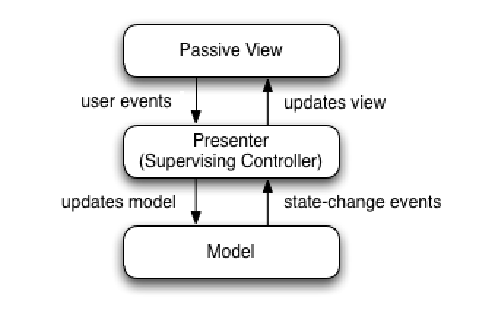
\includegraphics{./img/MVP.pdf}
\caption{Visualisierung des MVP Patterns \cite{bib:MVP1}}\label{Fig:MVP}
\end{center}
\end{figure}\\
Der Presenter übernimmt die Logik und die View ist einfach gehalten
\cite{bib:MVP2}. Dies sorgt für eine klare Trennung zwischen Model und View (vgl.
Abbildung \ref{Fig:MVP}). Bei MVC hingegen kennt die View das Model.
\cite{bib:MVCvsMVP}. Der Presenter steuert die View und übermittelt die Daten
des Model's zur View.
Daher wird der einfache Austausch von Views ermöglicht ohne das weitere
Änderungen vorgenommen werden müssen \cite{bib:MVP1}\cite{bib:MVP2}.

In der zu generierenden Anwendung soll dieses Pattern ohne ein Model
implementiert werden, da der Fokus ausschließlich auf eine GWT Frontend
Anwendung gerichtet ist. Die MVP Struktur ist dabei so umgesetzt, sodass der
Presenter als Interface in dem View Interface und konkret über die Activity
definiert wird. Die Activity regelt zusätzlich das Event Handling und die
Datenbeschaffung. Die View Implementierung beinhaltet eine
Instanz des Presenters, damit die Aktionen der View Komponenten
(bei GWT Widgets genannt) an den Presenter übergeben und dadurch an die
Activity weitergeleitet werden.

\subsection{UiBinder}
\label{UiBinder}
Das UiBinder Framework für GWT Anwendungen ist ähnlich zu betrachten wie HTML
und CSS. Dieses Framework ermöglicht das Layouting von GWT Websites. Dabei
wird die Website nicht nur über den Code erzeugt, sondern zusätzlich mittels
einer xml-Datei, die ui.xml Datei. In dieser Datei können innerhalb eines ui:Style
Tags (vgl. Listing \ref{lst:BSPCodeUIXML}) Style
Eigenschaften ähnlich wie bei CSS gesetzt werden. Dies bietet die Möglichkeit die
View Implementierung zu entkoppeln. Darüber hinaus existieren noch weitere
Möglichkeiten zur Entkopplung der View Implementierung, sodass z.B.
statische View Komponenten nur innerhalb der ui.xml
Datei enthalten sind und somit ein Overload der View Implementierung vermindert
werden kann. Weiterhin können die Komponenten innerhalb dieser Datei gebunden
werden an die Komponenten in der View Implementierung \cite{bib:uiBind}. Dazu
folgender Codeauszug von einem vorangegangenem GWT Projekt zur Erläuterung dieses Zusammenhangs.\\
\lstset{language=gwt}
\begin{lstlisting}[caption={Beispielcode UiBinder in View
Implementierung}, label={lst:BSPCodeView}]
	private static LoginViewImplUiBinder $uiBinder$ = GWT
			.create(LoginViewImplUiBinder.class);

	interface LoginViewImplUiBinder extends 
			UiBinder<Widget, LoginViewImpl> {}

	|@UiField|
	TextBox $name$;
		
	//Constructor
	|@Inject|
	public LoginViewImpl() {
		$content$.add($uiBinder$.createAndBindUi(this));
	}
	|@UiHandler|({ "button" })
	void onButtonPressed(ClickEvent e) {
		// do something
	}
\end{lstlisting}
\lstset{language=uixml}
\begin{lstlisting}[caption={Beispielcode UiBinder in ui.xml},
label={lst:BSPCodeUIXML}]
<!DOCTYPE ui:UiBinder SYSTEM 
	"http://dl.google.com/gwt/DTD/xhtml.ent">
<ui:UiBinder xmlns:ui="urn:ui:com.google.gwt.uibinder"
	xmlns:g="urn:import:com.google.gwt.user.client.ui"
	xmlns:my="urn:import:myprojectpackage">
	<ui:style>
		.enterbutton {
			font-size: 16px;
			font-weight: bold;
			padding: 10px;
			color: #336699;
		}
	</ui:style>
	<g:FlowPanel>
		<g:Label text="Anmeldename"></g:Label>
		<g:TextBox ui:field="name"></g:TextBox>
		<g:Button text="Einloggen" ui:field="button" 
			styleName="{style.enterbutton}"></g:Button>
	</g:FlowPanel> 
</ui:UiBinder> 
\end{lstlisting}
Die Annotationen @UiField und @UiHandler in der View Implementierung (vgl.
Listing \ref{lst:BSPCodeView}) ermöglichen den Zugriff auf die View Komponenten
mit dem jeweiligem Attribut ui:field in der ui.xml (vgl. Listing
\ref{lst:BSPCodeUIXML}). @UiField ist dabei dafür zuständig die Instanz zu
erhalten. Diese kann dann z.B. über den Java Code definiert oder Style
Eigenschaften gesetzt werden. Entgegen dem ermöglicht @UiHandler die Anmeldung
einer Methode auf der Instanz. Darüber kann dann im Falle des Beispiels ein
Klick Event auf dem Button ausgeführt werden.

Damit zeigen die Listings \ref{lst:BSPCodeView} und \ref{lst:BSPCodeUIXML}
nur kleine Beispiele für die Nutzung von dem UiBinder Framework, welche
innerhalb des Generator Projektes umgesetzt werden sollen.




% ---------------------------------------------
% GIN
% ---------------------------------------------
\section{Dependency Injection mittels GIN}
\label{GIN}
\chapter{Konzeption}
\label{Konzeption}
In erster Linie soll eine GWT Frontend Anwendung generiert werden, basierend auf
einer vorgegebenen Architektur (vgl. Abschnitt \ref{AufBZielArchitektur}). Dabei
ist eines der Hauptziele die leichte Erstellung der GWT Anwendung, ohne
Abhängigkeiten zu der zu generierenden Architektur. Darüber hinaus sollen
Vorteile durch vorgegebene Architekturpatterns wie der leichte Austausch von
View Implementierungen durch MVP weiterhin nutzbar sein. Zusätzlich ist es
wünschenswert, das Verhalten von View Komponenten wie Buttons beispielsweise für eine Navigation
zwischen den Webseiten zu ermöglichen. Weitere dieser Verhaltensspezifikationen
können das Öffnen eines Popups sowie die Übertragung von Daten sein. Auch hierbei
steht die einfache Erstellung einer GWT Anwendung und die Konformität
der Architektur im Vordergrund.

Es sollen alle von GWT vorgegebenen View Komponenten wie Label und
Menus für den Entwickler verwendbar sein, welche zusätzlich
untereinander zugeordnet werden können. Des Weiteren sollen Elemente, die auf
jeder Webseite zu sehen sind, wie z.B. ein Header implementiert werden. Layout-
und Stylevorgaben sollen nicht berücksichtigt werden, da dafür UI Editoren
existieren.

Es sollen weitere eigene View Komponenten, z.B. eine Datentabelle, die mehrmals
verwendet wird, erstellt werden können, damit, unabhängig der vorgegebenen
Architektur, weitere architektonische Maßnahmen erfolgen können. Darüber hinaus soll
eine vorgegebene sowie eine durch den Nutzer erstellte Paketierung
für Views generiert werden.

Zur Erstellung einer GWT Frontend Anwendung soll ein UML Modell auf M1 Ebene
erstellt werden (vgl. Abschnitt \ref{AufBM1}), basierend auf dem zum
Generator Projekt gehörendem UML Profil auf M2 Ebene (vgl. Abschnitt
\ref{AufBProfil}), welches durch den Generator (vgl. Abschnitt \ref{AufBGenerator}) mittels
MTL generiert werden soll.
% ---------------------------------------------
% Konzepte
% ---------------------------------------------
% ---------------------------------------------
% ZielArchitektur
% ---------------------------------------------
\section{Ziel-Architektur}\label{AufBZielArchitektur}
Die für die Generierung vorgesehene Architektur basiert auf 
Architekturkonzepten verschiedener Entwickler und entstand bei der Entwicklung
von vorhergehenden GWT Projekten. Diese Architektur stellte sich dabei als Best
Practice Lösung heraus, welche jedoch aufwändig und fehleranfällig bei der
Umsetzung ist. Dies ist einer der Gründe einen Generator für GWT Frontend
Anwendungen zu entwickeln. Im Folgendem wird die umzusetzende Architektur
kategorisiert und anhand der zu erstellenden Klassen und Dateien vorgestellt.
% -------------------Struktur Erklärungen--------------------------
\begin{itemize}
  \item einmalig vorhandene Dateien und Klassen
  \begin{itemize}
    \item \textbf{index.html}\\
    HTML Seite über die, durch GWT, die in Java erzeugten View Klassen
    eingebunden werden.
    \item \textbf{styles.css}\\
    CSS Datei für die Festlegung der Style-Eigenschaften.
    \item \textbf{\grqq{}Name\grqq{}.gwt.xml}\\
    Konfigurationsdatei in der u.A. verwendete Bibliotheken sowie
    Browsereinstellungen und die Zugriffsklasse eingetragen wird.
    \item \textbf{AppEntryPoint.java}\\
    Zugriffsklasse, d.h. die Einstiegsklasse für die GWT Anwendung. In dieser
    Klasse wird u.A. die ContentView sowie die PermanentViews und die
    HistoryMapper definiert.
    \item \textbf{AbstractView.java}\\
    Ist die Oberklasse aller View Klassen Implementierungen innerhalb der
    esrtellten GWT Anwendung. Diese definiert Eigenschaften für alle Views und
    ermöglicht als Oberklasse den Austausch der
    Ansichten.-----------------------------------
    \item \textbf{AbstractActivityDefaultImpl.java}\\
    Diese Klasse wird von allen View Activity Klassen erweitert und dient
    mittels \textit{start}-Methode dazu die View Klassen aufzurufen und dem
    Zugriff auf die Views über den Browser mittels \textit{Place}.---------
    \item \textbf{\grqq{}Name\grqq{}ViewActivityMapperImpl.java}\\
    Definiert die \textit{PlaceControllerProvider} damit darüber der View Place
    aufgerufen werden kann und somit im Browser die View Implementierung
    erscheint. Diese Klasse existiert prinzipiell einmal. Kommt jedoch eine
    PermanentView hinzu so kommt je PermanentView eine weitere
    ViewActivityMapper-Implementierung dazu, welche sich jeweils ihren
    PermanentViewActivity als \textit{PlaceControllerProvider}
    definiert. Diese \textit{PlaceControllerProvider} werden
    dann nicht in der ursprünglich existierenden
    ViewActivityMapper-Implementierung definiert.-----------------
    \item \textbf{AppPlaceHistoryMapper.java}\\
    Ermöglicht über die View Places den Zugriff auf die gezeigte View
    Implementierung durch den Back-Button im Browser oder innerhalb der View
    Implementierung nachdem dies in der View Activity implementiert wurde.
    \item \textbf{AppGinjector.java}\\
    Über diese Java Klasse wird es u.A. ermöglicht die
    ViewActivityMapper-Implementierungen sowie den EventBus zu
    erhalten, welcher die Navigations-Historie enthält bzw. speichert. Darüber
    können diese weiterhin in dem \textit{AppEntryPoint} definiert werden.
    \item \textbf{PlaceControllerProvider.java}\\
    Ist die Schnittstelle zu den View Places. Damit können diese in der
    ViewActivityMapper-Implementierung aufgerufen werden und dadurch der Zugriff
    auf die View Implementierungen zur Ansicht im Browser ermöglicht werden.
    Dies wird über die Einbindung von GIN ermöglicht.
    \item \textbf{ProductionGinModule.java}\\
    In dieser Klasse werden die für GIN typischen bind-Befehle definiert. Diese
    dienen u.A. dazu die View Interfaces an die View Implementierungen zu
    binden, sowie die Start-View festzulegen.
  \end{itemize}  
  \item View Klassen und Dateien, welche für jede View implementiert werden,
  basierend auf dem MVP-Pattern
    \begin{itemize}
    \item \textbf{\grqq{}Name\grqq{}Activity.java}\\
    Dient der Implementierung des Presenters sowie der Definierung der View.
    Darüber hinaus wird innerhalb dieser Klasse der PlaceController definiert,
    worüber u.A. eine Navigation zwischen den Webseiten im Browser erfolgen kann
    mittels einer \textit{goTo}-Methode.
    \item \textbf{\grqq{}Name\grqq{}Place.java}\\
    Diese Implementierungen sehen im groben inhaltlich immer gleich aus. Die
    Unterscheidung ist hierbei die dazugehörige View. Über diese Klasse wird die
    Navigation innerhalb der Seiten bzw. View Implementierungen ermöglicht.
    \item \textbf{\grqq{}Name\grqq{}View.java}\\
    Hierbei handelt es sich um ein Interface, welches des Presenter Interface
    enthält und ist die Oberklasse für die jeweiligen View Implementierungen.
    Diese Schnittstelle ermöglicht den einfachen Austausch der verschiedenen
    View Implementierungen für die Anwendung, welches zusätzlich über einen
    \textit{bind}-Befehl innerhalb des \textit{ProductionGinModule} festgelegt
    werden muss.
    \item \textbf{\grqq{}Name\grqq{}ViewImpl.java}\\
    Dabei handelt es sich um die konkreten View Implementierungen, welche im
    Browser sichtbar sind. Diese implementieren die jeweilige View und enthalten
    den durch die View und Activity implementierten Presenter, wodurch die
    Kontrolle der View Implementierung seitens des MVP-Prinzips abgegeben wird.
    Darüber hinaus kann diese Klasse die notwendigen View Komponenten
    definieren, wenn dies erforderlich, z.B. zum Befüllen von Datentabellen,
    oder dies gewünscht, z.B. zum Zugriff auf Buttons oder zur inhaltsabhängigen
    Erstellung von View Komponenten, ist. Die View Implementierung ist an
    eine bestimmte fest definierte
    \textit{\grqq{}Name\grqq{}ViewImpl.ui.xml}-Datei gebunden, durch die Angabe
    des gleichen Namens \grqq{\grqq{}Name\grqq{}ViewImpl}\grqq. Zusätzlich
    können durch die Annotation \textit{@UIField} die View Komponenten der
    \textit{\grqq{}Name\grqq{}ViewImpl.ui.xml}-Datei innerhalb der
    View Implementierung aufgerufen und definiert werden.
    \item \textbf{\grqq{}Name\grqq{}ViewImpl.ui.xml}\\
    Innherhalb dieser Datei können Style-Eigenschaften zu den View Komponenten
    sowie die View Komponenten definiert werden.-----------
  \end{itemize} 
  \item View Klassen und Elemente die auf jeder Ansicht zu sehen sind:
    \begin{itemize}
    \item werden auch nach dem MVP Pattern, wie oben beschrieben, erstellt.
    \item innerhalb des AppEntryPoint enthalten und definiert.
    \item bilden jeweils eine eigene
    \textit{\grqq{}Name\grqq{}ViewActivityMapper} Implementierung.
  \end{itemize} 
\end{itemize}

% -------------------View Eintragungen--------------------------
Basierend dieser Architektur muss zur Erzeugung einer View, diese eingetragen
werden innerhalb der der folgenden Klassen:
    \begin{itemize}
    \item \grqq{}Name\grqq{}ActivityMapperImpl.java
    \item AppPlaceHistoryMapper.java
    \item ProductionGinModule.java
  \end{itemize} 
und folgende Klassen und Dateien erzeugt werden:
   \begin{itemize}
    	\item \grqq{}Name\grqq{}Activity.java
    	\item \grqq{}Name\grqq{}Place.java
    	\item \grqq{}Name\grqq{}View.java
    	\item \grqq{}Name\grqq{}ViewImpl.java
    	\item \grqq{}Name\grqq{}ViewImpl.ui.xml
  \end{itemize} 
unter Betrachtung, dass ausschließlich eine View Implementierung existiert.
Existieren zu einer View mehrere View Implementierungen so müssen mehrere
Eintragungen innerhalb des \textit{ProductionGinModule.java} getätigt werden und
mehrere \textit{\grqq{}Name\grqq{}ViewImpl.java} und
\textit{\grqq{}Name\grqq{}ViewImpl.ui.xml} erstellt werden. Dadurch wird eine
gute Abstraktion und lose Kopplung geschaffen. Dies ist jedoch sehr
aufwändig und fehleranfällig, da leicht ein Eintrag vergessen werden kann und
viele Klassen erzeugt werden müssen.

% -------------------Packages--------------------------
Zu den genannten Architekturvorstellungen gehört zusätzlich eine Paketierung,
die auch durch vorherige GWT-Projekte entstand. Der Vorteil der folgenden
Gliederung der Pakete besteht darin, dass innherlab der
\textit{\grqq{}Name\grqq{}.gwt.xml} Konfigurationsdatei das source-Tag, welches
den Pfad für den zu übersetzenden Java Code angibt, wie folgt: $<source
path='client'/>$ definiert werden kann. Folgend die Gliederung der Klassen
innerhalb ihrer Packages:
\begin{itemize}
  \item \grqq{}projektname\grqq{}
  	\begin{itemize}
    	\item \grqq{}Name\grqq{}.gwt.xml
  	\end{itemize}
  \item \grqq{}projektname\grqq{}.client
    \begin{itemize}
    	\item AppEntryPoint.java
    \end{itemize}
  \item \grqq{}projektname\grqq{}.client.common
    \begin{itemize}
      	\item AbstractView.java
  	  	\item AbstractActivityDefaultImpl.java
    	\item \grqq{}Name\grqq{}ViewActivityMapperImpl.java
    	\item AppPlaceHistoryMapper.java
    \end{itemize}
  \item \grqq{}projektname\grqq{}.client.gin
    \begin{itemize}
   		\item AppGinjector.java
    	\item PlaceControllerProvider.java
    	\item ProductionGinModule.java
    \end{itemize}

  \item \grqq{}projektname\grqq{}.client.view
    \begin{itemize}
    	\item \grqq{}Name\grqq{}Activity.java
    	\item \grqq{}Name\grqq{}Place.java
    	\item \grqq{}Name\grqq{}View.java
    	\item \grqq{}Name\grqq{}ViewImpl.java
    	\item \grqq{}Name\grqq{}ViewImpl.ui.xml
	\end{itemize}
\end{itemize}
Jedoch soll für einen Entwickler die Möglichkeit bleiben innerhalb des view
Packages, die Views in Packages zu gliedern. Aus diesem Grund soll an dieser
Stelle das view Package nicht Generator-seitig tiefer gegliedert werden.

Anhand der beschrieben Architektur wird ersichtlich, dass die Erstellung eines
GWT Projektes hauptsächlich im Bereich der einmalig vorhanden Dateien und
Klassen und die Erstellung einer View im groben immer gleich ist. Dies bietet
zwar den Vorteil der Vereinheitlichung mehrerer GWT Projekte und gewährleistet
eine gewisse Übersichtlichkeit und kurze Einarbeitungszeit in verschiedenen GWT
Projekten, ist aber sehr aufwändig und fehleranfällig. Beispielsweise kann über
\grqq{}Copy-Paste\grqq{} viel esrtellt und implementiert werden, jedoch ist
dabei das Risiko erhöht, dass Einträge vergessen werden abzuändern oder
hinzuzufügen. Darüber hinaus kann es passieren, das Einträge enthalten sind wie
z.B. einer Bibliothek, welche jedoch nicht mehr benötigt werden und somit nicht
im Build-Path enthalten sind.
Diese Beispiele führen potenziell alle dazu, dass die gesamte GWT Anwendung nicht mehr startet
und die Suche nach dem Fehler erschwert wird, da oftmals viele dieser
Fehler flüchtig geschehen können. 
% ---------------------------------------------
% Profil
% ---------------------------------------------
\section{Profil}\label{AufBProfil}
Eines der Hauptziele ist wie erwähnt die erleichterte Erstellung von GWT
Projekten unter Nutzung der durch die Architektur gegebenen Vorteile. Zu welchen
auch der einfache Austausch von View Implementierungen unabhängig vom Model
gehört. Des Weiteren soll der Aufwand und die Fehleranfälligkeit bei der
Erstellung eines GWT Projektes sowie zur Erstellung von Views (vgl.
Abschnitt \ref{AufBZielArchitektur}) minimiert werden werden. Diese Ziele
erfordern einen hohen Abstraktionsgrad innerhalb des Profils sowie weiterhin des
M1-Modells.

Deswegen soll eine der ersten Überlegungen dazu führen, dass das
gesamte GWT Projekt auf ein gemeinsames Element reduziert werden soll. Dieses
Element erscheint im Rahmen des, aus der Architektur heraus, umzusetzenden
MVP-Patterns in dem die View Klassen und Dateien
\textit{\grqq{}Name\grqq{}Activity.java}, \textit{\grqq{}Name\grqq{}Place.java},
\textit{\grqq{}Name\grqq{}View.java}, \textit{\grqq{}Name\grqq{}ViewImpl.java}
und \textit{\grqq{}Name\grqq{}ViewImpl.ui.xml} das gemeinsame Element für alle
anderen Klassen und Inhalte bieten. Jedoch erschien dadurch der Aufwand bei der
Erstellung von Views nicht minimiert, da durch diese Stereotypenbildung, diese
im M1-Modell weiterhin Einsatz finden müssen. Aus diesem Grund ist eine weitere
Suche nach dem gemeinsamen Element erforderlich. Dies führt durch die, sich auch
in diesem Rahmen als vorteilhaft herausstellende, Architektur dazu, dass dies
das unterste Element ist, die \textbf{View Implementierung}.  Diese erscheint
ausreichend für die Erstellung der gesamten einmalig vorhandenen Klassen und
Dateien sowie der View Klassen und Dateien, da innerhalb der View
Implementierung und der simultanen und vereinheitlichten Namensbennenung alle
notwendigen Teile generierbar wären. 

Eine weitere Anforderung ist der Austausch der View Implementierungen durch den
Einsatz von MVP. Dieser kann jedoch nicht ausschließlich durch die View
Implementierung erfolgen, da hierbei eine Möglichkeit gegeben werden muss zu der
Verbindung meherer View Implementierungen zueinander. Aus diesem Grund soll das
\textbf{View Interfaces} genutzt werden. Dies stellt die Verbindung von mehreren
View Implementierungen in Form einer Oberklasse her. Zusätzlich bietet dies die
Möglichkeit bestimmte Methoden zu definieren, welche für jede implementierende
View nützlich ist. 

View Implementierungen haben zusätzlich View Komponenten und darüber hinaus ist
die Umsetzung einer Navigation bzw. das Verhalten bei Interaktion mit
View Komponenten ein weiteres umzusetzendes Ziel. In vorhergehenden Generator
Projekten ging die Umsetzung dessen mittels Enumerations hervor. Diese sind
sinnvoll wenn eine View Komponente mehere Attribute z.B. eine Value haben soll
und kein konkreter Nachbau von bestehenden Frameworks erfolgen soll. In dem Profil
wird ein hoher Abstraktionsgrad erwartet, damit eine Vereinfachung gewährleistet
werden kann. Deswegen bildet der Einsatz von Enumerations als Typ für
View Komponenten einen Mehrwert für die Umsetzung des Profils. Zusätzlich wird ein Layouting als
Ziel ausgeschlossen, wodurch die Nachteile der Verwendung von Enumerations
verringert werden. Dadurch ergibt sich zusätzlich der Einsatz von \textbf{View
Komponenten} als Stereotypen mit dem Attribut \textit{type} vom Typ
\textbf{Enumeration View Objekt Typ}.

Für Navigationselemente wie Buttons und Umsetzung der Navigation ist eine
Überlegung ein weiteres Profil für ActivityDiagramme und somit ein
ActivityDiagramm als M1 Modell zu nutzen. Dieses Mittel ermöglicht eine
Übersicht über die Navigationsstruktur bzw. Verhaltensstruktur einer Anwendung
und ist somit gut geeignet. Dennoch ist das Ziel der Vereinfachung nicht
gegeben, da für jedes Navigationselement ein extra Eintrag in einem
ActivityDiagramm erfolgen muss und somit eine Redundanz innerhalb der
verschiedenen M1-Modelle entsteht und der Mehrwert der Navigationsgenerierung
seitens des Entwicklers, welcher das Generator Projekt nutzen möchte, mindert
aufgrund des Mehraufwandes. Die Verwendung von Enumerations für View Objekte
ermöglichte die Idee, dass für navigierbare bzw. verhaltensbasierte Elemente
eine ähnliche Handhabung dienlich sein kann. Diese ermöglichen die Erfüllung der
Zielsetzung und bieten über die Angabe eines Attributes \textit{goTo} die
Navigation sowie über weiterer Attribute z.B. \textit{openPopup} eine
Generierung verhaltensbezogener Inhalte über das M1-Modell. Dies führt zu der
Stereotypenbildung der \textbf{Navigations View Komponenten} mit
\textbf{Enumeration Navigations View Objekt Typen}. Diese Enumeration enthält
dann z.B. Tree, Button oder MenuBar, d.h. View Komponenten von GWT, welche für
Navigationen oder Verhaltensspezifikationen vorgesehen sind.

\textbf{Navigations View Komponente} und \textbf{View Komponenten} sind
Properties, da eine View Implementierung diese View Komponenten enthalten kann.

Zur Kopplung von großen Views und zur Erweiterung der vorgegebenen Mittel anhand
der Architektur soll eine weitere Klasse als Stereotyp dienen, die
\textbf{eigenen View Komponenten}. Darin sollen bestehende View Komponenten
enthalten sein und somit eine eigene View Komponente, z.B. eine große
Datentabelle, bilden, die innerhalb einer View Implementierung enthalten sein
kann.

Im Bereich von Views z.B. ein Header die auf allen Views innerhalb des Browsers
sichtbar sind, soll eine weiterer Stereotypenbildung stattfinden. Diese Views
sind \textbf{Permanente Views} und gliedern sich zusätzlich in \textbf{Header}
und \textbf{Footer}, da diese konkrete permanente Views sind durch ihre
Positionierung in einer View (Header oben, Footer unten). Diese Views verhalten
sich simultan zu den normalen Views, weshalb die permanenten Views als View
Implementierung von dem View Interface umgesetzt werden können. Dadurch wird
zusätzlich der Austausch von View Implementierungen ermöglicht.
% ---------------------------------------------
% M1-Modell
% ---------------------------------------------
\section{M1-Modell}\label{AufBM1}
Basierend auf dem UML-Profil soll das Modell View Implementierungen enthalten,
welche wiederum View Komponenten als Properties beinhalten können sowie eigene
View Objekte zu diesen zugeordnet sein können. Darüber hinaus sollen über
Attribute innerhalb von Navigations View Komponenten, im M1-Modell enthaltene,
View Implementierungen angegeben werden, sodass z.B. über das Attribut goTo die
Navigation zu dieser View Implementierung durch Generierung erfolgen kann.
Darüber hinaus sollen permanente View Implementierungen in Form z.B. eines
Headers erstellt werden, welche dann auf jeder View innerhalb des Browsers
sichtbar sind. Eine Implementierung eines Headers soll eine MenuBar enthalten,
die durch MenuItems die Navigation zu verschiedenen Seiten ermöglicht.
Zusätzlich sollen, z.B. für die Implementierung einer GWT Anwendung, für
verschiedene Devices z.B. einen Browser auf einen Desktop oder einem Browser auf
einem Smartphone, View Intefaces rstellt werden, welche mehrere
Implementierungen haben, sodass diese für verschiedene Devices ausgelegt angezeigt werden.
% ---------------------------------------------
% Generator
% ---------------------------------------------
\section{Generator}\label{AufBGenerator}
Im Bereich des UML-Profils sowie des M1-Modells sind außer der Views und ihren
Implementierungen und ihren View Komponenten die weiteren Klassen und Dateien
ungeachtet geblieben. Aus diesem Grund muss der Generator so geschrieben werden,
sodass aus dem M1-Modell ein gesamtes GWT Projekt generiert werden kann. Dies
soll potenziell auch ermöglicht werden in dem nur eine View Implementierung
erstellt wird, welche ohne Attribute und Methoden ausgestattet ist. Dazu soll
eine Unterleitung erfolgen, welche einerseits die einmalig vorhandenen Klassen
mit Inhalten (auch View abhängiger Inhalte) generiert und andererseits die Views
generiert. Existieren View Interfaces so sollen die Klassen \textit{\grqq{}Interfacename\grqq{}View.java},
\textit{\grqq{}Interfacename\grqq{}Activity.java} und
\textit{\grqq{}Interfacename\grqq{}Place.java} den Interfacenamen tragen und die
Implementierungsklassen bzw. Dateien
\textit{\grqq{}Klassenname\grqq{}ViewImpl.java} und
\textit{\grqq{}Klassenname\grqq{}ViewImpl.ui.xml} der View, die
Implemntierungsklassennamen. Darüber hinaus sollen die View abhängigen Inhalte,
wenn mehr als eine View Implementierung vorhanden ist, mittels eines boolean
\textit{binding} dementsprechend unterschieden werden, sodass alle Inhalte
basierend auf View Implementierungen auskommentiert werden, bei binding gleich
false. Dadurch kann ein einfacher Austausch bei einem Wechsel
der View über das MVP-Pattern ermöglicht werden, ohne Code hinzufügen zu müssen.
In dem Fall, dass kein View Interface zu einer Implementierung gehört, so werden
alle Klassen, Dateien und View abhängige Inhalte mittels des
Implementierungsklassennamen generiert.

Für alle Permanenten Views gilt ein
ähnliches Vorgehen wie bei den normalen Views. Jedoch haben diese die
Besonderheit, dass sie in jeder View zu sehen sind und somit zusätzlich zu der
einen \textit{AbstractView} in dem \textit{AppEntryPoint.java} eingetragen
werden. Dazu erfolgt eine durch das Profil vorgegebene Unterscheidung zwischen
normalen permanenten Views und Header und Footer. Da Header (oben) und Footer
(unten) eine feste Positionierung auf einer Webseite haben, werden diese durch
den Generator dementsprechend in dem \textit{AppEntryPoint.java} positioniert.
Alle anderen vorhandenen permanenten Views sollen dazwischen eingetragen werden
und müssen später durch den Entwickler positioniert werden, da dies
layoutspezifisch ist.

Der Entwickler soll weiterhin zusätzliche Änderungen vornehmen müssen bzgl. der Startseite der GWT
Webanwendung, welches in dem generiertem Code anstatt
konkreter Angabe des Klassennamens innerhalb des Befehls über
\grqq{}Start\grqq{} gekennzeichnet wird. Dieses Vorgehen kann das Verständnis
für die Architektur stärken und es werden überflüssige und überfüllende
Attribute innerhalb des Profils und M1-Modells vermieden.

allg. zum Generator z.B. Strukturierung, Redundanz usw.
\section{Anwendungsfall}
\label{Anwendungsfall}
Prinzipiell soll es über den Generator möglich sein verschiedene Anwendungsfälle
zu generieren. Beispielhaft soll dementsprechend eine
einfache Homepage mit u.A.
einem Portfolio und einer Newsseite sowie einem Header über dem alle Seiten
erreichbar sind als Anwendungsfall dienen. Weiterhin soll mit 2
M1-Modellen gearbeitet werden, in dem der Anwendungsfall inhaltlich leicht abgeändert wird.
Ein M1-Modell dient Testzwecken und das andere der Vervollständigung der
gesamten Homepage mit Änderungen in dem generiertem Code z.B. zur Gestaltung der
Homepage und einer vollständigen und geordneten Projektstruktur.
Dadurch können alle Test- und verschiedene Anwendungsfälle abgedeckt werden,
inklusive der Einbindung von View Komponenten, und eine Trennung zwischen notwendigen Änderungen im
generiertem Code, durch ein einheitliches Projekt, erfolgen.
\chapter{UML Profil auf M2 Ebene}
\label{UMLProfil}
In diesem Projekt wurde vorab entschieden, den bestehenden Sprachumfang der UML durch UML-Profile zu erweitern. Ein UML-Profil ist genau genommen eine Erweiterung dessen Metamodells und somit des Standard Sprachumfangs der UML und es ist gleichzeitig ein UML-Modell.

Das UML Profil wird mit eigens definierten Meta Klassen erweitert. Grund hierfür ist, dass im späteren UML Modell Zuständigkeiten besser zugewiesen und erkannt werden können.
Diese Erweiterungen werden als Stereotype im Profil bezeichnet, die von vordefinierten Metaklassen abgeleitet werden.

Im folgenden is die Endfassung des Profils zu sehen, welche anschließend genauer erläutert wird.
\begin{figure}[htbp]
\begin{center}
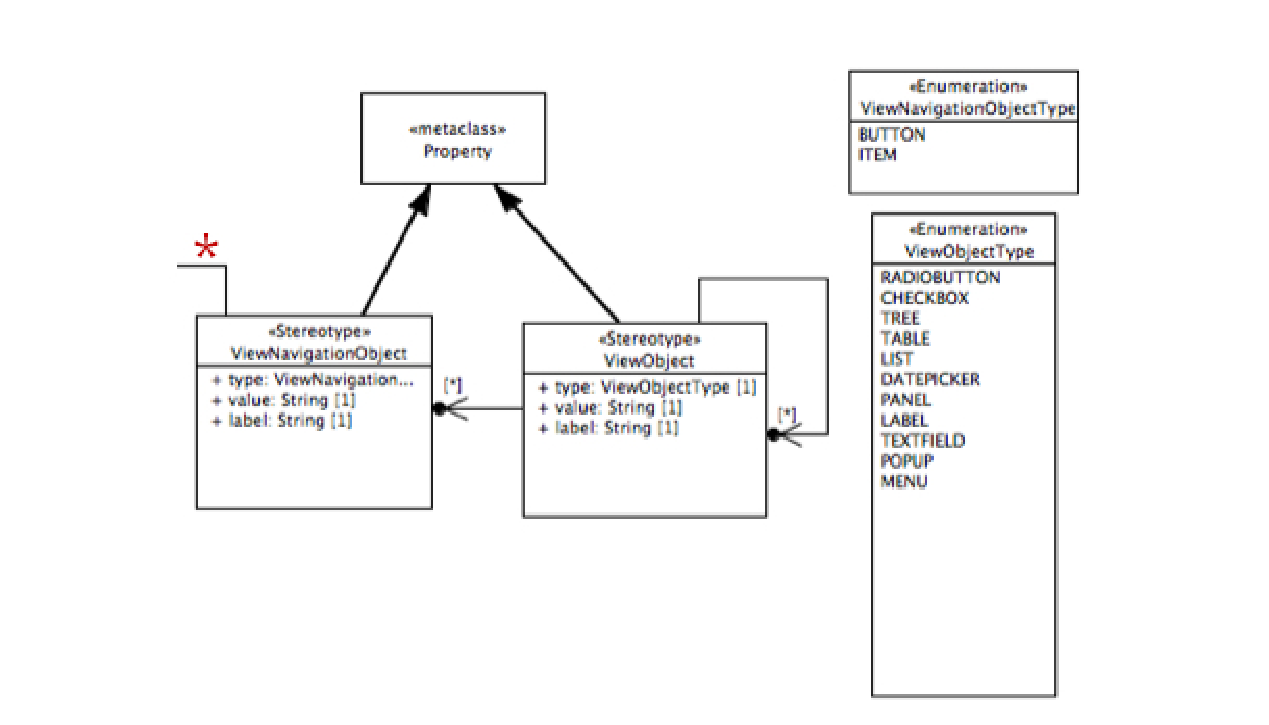
\includegraphics[width=\textwidth]{./img/ProfilProp.pdf}
\caption{Darstellung der Properties und Enumerations im Profil}\label{Fig:UMLProfil}
\end{center}
\end{figure}\\
In dem Profil wurden zwei Stereotypen für Properties definiert. Die \textbf{ViewObject} und die \textbf{ViewNavigationObject}, die die Widgets in GWT repräsentieren. Durch die Frontendbetrachtung gibt es nur Elemente, die entweder zum Anzeigen von Informationen ( \textbf{ViewObject}) oder zum Navigieren auf andere Views (ViewNavigationObject) dienen. Die Trennung der doch ziemlich ähnlichen Elemente musste erfolgen, da es nur so möglich wurde, dass zwar  \textbf{ViewObjects} andere  \textbf{ViewObjects} oder  \textbf{ViewNavigationObjects} enthalten können, bei  \textbf{ViewNavigationObjects} dies wiederum aber nicht möglich sein darf. 
Im Sinne einer besseren Übersichtlichkeit wurde sich darauf geeinigt, den Typ der Property mit Hilfe von Enumerations festzulegen. Diese ermöglichen eine Reduzierung der unterschiedlichen Modellelemente. Es wurde hierbei bewusst auf die Darstellung der Widget als eigene Klassen verzichtet, um es später für den GWT Entwickler einfacher zu gestalten. Im Unterschied zur Konzeption wurde festgelegt, dass Multi-Navigationselemente (wie Table, List, Menu oder Tree) als  \textbf{ViewObject} definiert sind, die dann wiederum ViewNavigationObjects von type  \textbf{ITEM} besitzen. Die Gruppierung als Items, die zuvor in der Konzeption als Menuitems oder treeitems aufgeführt wurden, ermöglichte es, die Generierung einfacher zu gestalten. Denn alle Items konnten nun gleich generiert werden, unabhängig davon, welchem  \textbf{ViewObject} sie angehören.\\

Bei den Widgets lag aus Zeitgründen der Fokus auf den jeweils wichtigsten Elementen ( \textbf{BUTTON},  \textbf{ITEM},  \textbf{TEXTFIELD},  \textbf{TABLE} etc.), da im späteren Verlauf des Projektes auch alle Elemente generierbar sein sollten. Dies lässt sich aber in zukünftigen Versionen einfach erweitern, indem man zusätzliche Enumerations hinzufügt und die Erstellung dieser im Generator anpasst. 
Weitere Attribute wie value oder label wurden dann in dem entsprechenden Stereotype als Attribut hinterlegt.
Hierbei ist anzumerken, dass das ViewNavigationObject in der ersten Fassung noch ein zusätzliches Attribut goToView besaß. Im Verlauf der Implementierung des Generators, stellte sich das als fehlerhaft heraus, da dies eine 1:1 Beziehung beschrieb und eine View nur von einem einzigen ViewNavigationObject angesteuert werden konnte. Um dieses Problem zu beheben, wurde eine Assoziation im Profil hinzugefügt. So ist es jetzt beispielsweise möglich, dass unterschiedliche Impressum-Buttons auf die gleiche ViewImpl Impressum verweisen können. \\
\begin{figure}[htbp]
\begin{center}
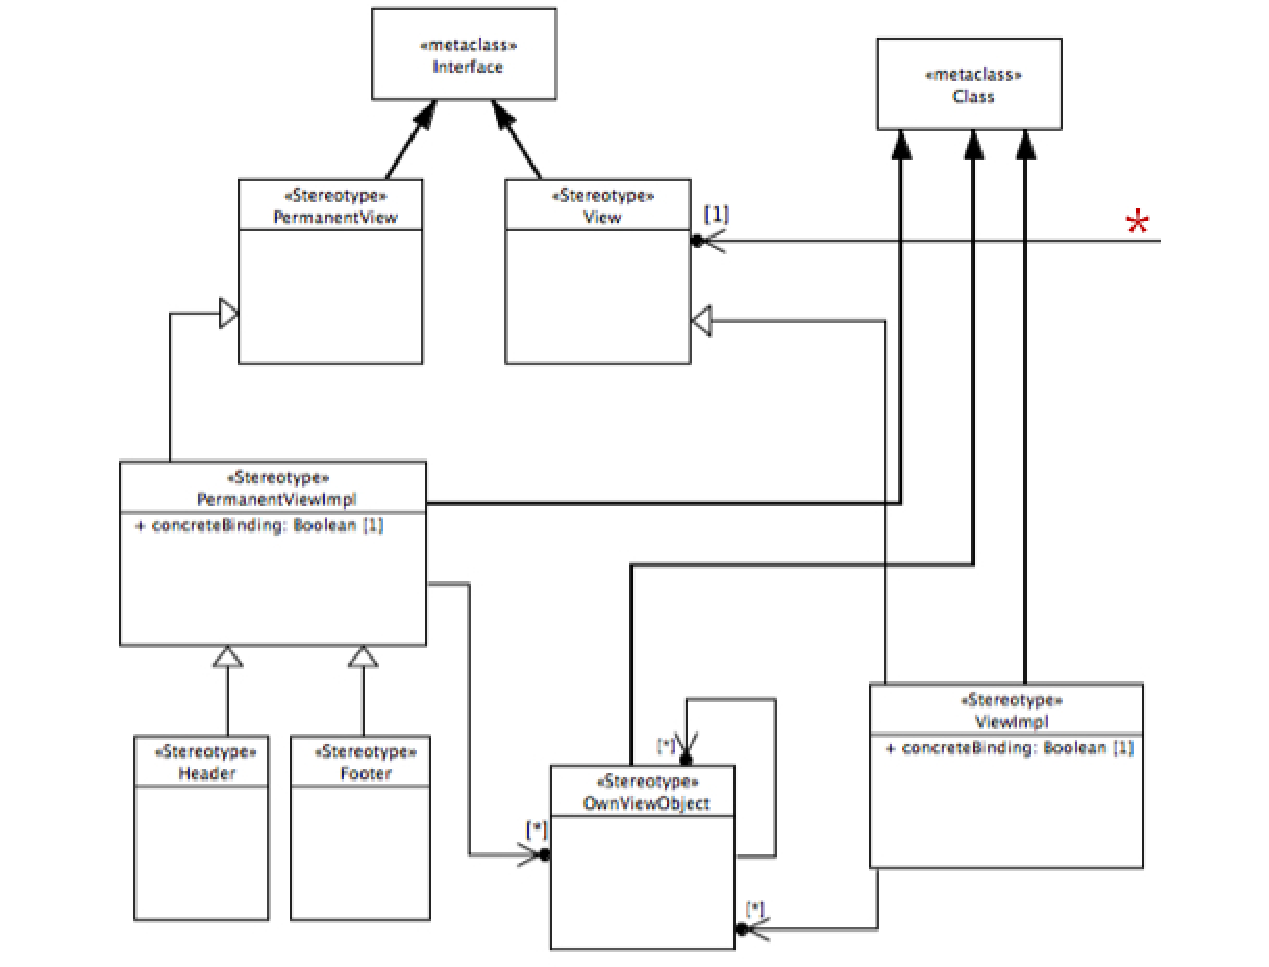
\includegraphics[width=\textwidth]{./img/ProfilClass.pdf}
\caption{Darstellung der Classes und Interfaces im Profil}\label{Fig:UMLProfil}
\end{center}
\end{figure}\\

Es wurden die Stereotypen  \textbf{View} und eine statische  \textbf{PermanentView} von der Metaklasse Interface abgeleitet. Diese bieten eine hilfreiche Schnittstelle für deren Implementationen. Die beiden Interfaces werden als Stereotype  \textbf{ViewImpl} und  \textbf{PermanentViewImpl} der Meta Klasse class implementiert. Durch Erstellen des Boolean - Attributs \textbf{concreteBinding} ist es möglich, den entsprechenden bind-Befehl über den Generator zu setzen. Da im Regelfall kein Interface besteht oder es nur eine Implementierung von einem speziellen Interface gibt, ist dieser Wert per Defaultwert auf true gesetzt. In diesem Fall gib es immer nur diese eine spezielle View, die angezeigt werden kann. Sollte es aber mehrere Implementierungen zu einem Interface geben, muss das  \textbf{concreteBinding}  dieser per Hand angepasst werden. Dadurch wird dieses im Anwendungsfall entsprechend gesetzt und gleichzeitig nur die richtige View ausgewählt.
Anfangs gab es für die Interfaces mehrere Lösungsansätze. In der ersten Fassung beispielsweise erbten auch  \textbf{Footer}  und  \textbf{Header}  direkt vom \textbf{PermanentView} Interface. Da  \textbf{Footer} und  \textbf{Header} aber eigentlich \textbf{PermanentViewImpl} mit vordefinierten, festen Positionen sind, war es sinnvoller diese direkt von der \textbf{PermanentViewImpl} erben zu lassen. So wie es letztendlich in der Endfassung auch umgesetzt wurde.  \\

Für spezielle Klassen wurde noch der Stereotype \textbf{OwnViewObject} hinzugefügt, der es dem Entwickler später ermöglichen soll, als Hülle für mehrere unterschiedliche \textbf{ViewImpl} oder auch \textbf{PermanentViewImpl} zur Verfügung stehen soll. Es dient somit als eigenständiges Widget, das aber die Möglichkeit bietet andere GWT Widgets zu enthalten.

Damit auch hier der Umfang des Arbeitsaufwandes für den GWT Entwickler so gering wie möglich gehalten wird, wurden im Profil die Stereotypen, wie von GWT vorgesehen, Activity und Place nicht angelegt. So müssen sich die Entwickler im M1 Modell zu diesen Klassen keine Gedanken mehr machen, denn mit Hilfe des Generator werden diese automatisch zur entsprechenden View generiert. 
Auch der direkte Stereotype Model, welcher beispielsweise die Schnittstelle zu einer Datenbank repräsentiert hätte, entfällt in dem Profil. Im Projekt war diese Backend-Anbindung nicht vorgesehen. Daten können später direkt in dem UML M1 Modell angegeben werden oder über XML Dateien geladen werden.
\chapter{Aufbau und Struktur M1 Modell} \label{M1Modell}
Beim M1 Modell handelt es sich um die direkte Darstellung der zu generierenden
Seiten für die Webanwendung. Dieses Modell wird direkt durch den Generator,
siehe Abschnitt \ref{Generator}, umgesetzt und um alle zusätzlichen Dateien
erweitert, die für die Zielarchitektur notwendig sind. In dem, in dieser Arbeit,
beschriebenen Generator, ist es nicht vorgesehen ein Projekt vollständig, mit
allen Einzelheiten, zu modellieren und erzeugen zu können, aus diesem Grund ist
auch das M1 Modell nicht als vollständige Abbildung für das Projekt zu
verstehen, das Ziel lag vor allem darauf die Architektur mit möglichst wenig
aufwand für den Entwickler zu generieren.

In dieser Arbeit, soll der Generator aus dem M1 Modell, eine möglichen
Grundstruktur für ein GWT Projekt erzeugen, welches dur kleine änderunge
lauffähig ist. Das M1 Modell ist so angedacht, dass alle Seiten eine
eigenständige Klasse darstellen. Des Weiteren können einfache Elemente, wie
Beispielsweise Label und Textfelder den Seiten hinzugefügt werden.
Zu dem ist es möglich die Navigation zwischen den Seiten, beispielsweise mit
Hilfe eines Menüs, in das Modell mit einzubringen. 

Durch die Verwendung eines Profils sind in dem M1 Modell keine Assoziationen
zu sehen. Dies sorg dafür, dass keine Verbindung zwischen den einzelnen Seiten
zu sehen ist. Die Navigation wird ausschließlich über die Properties der
Navigations Elemente erstellt, in dieser Arbeit mit
\textit{viewNavigationObject} benannt. Dies sorgt für eine leichtere Erstellung
dessen Im M1 Modell durch den Entwickler, erschwert allerdings das Erkennen
der Navigation.

\section{M1 Modellaufbau}
Wenn ein neues Projekt angelegt wird, muss in den Properties des M1 Modells
neben der Angabe des Profils, ein Name definiert werden. Dieser Name stellt
später den Hauptpaketnamen des GWT Projektes dar und legt somit den Grundstein
für die Paketstruktur (siehe Abbildung \ref{Fig:mainpackage}).

\begin{figure}[htbp]
\begin{center}
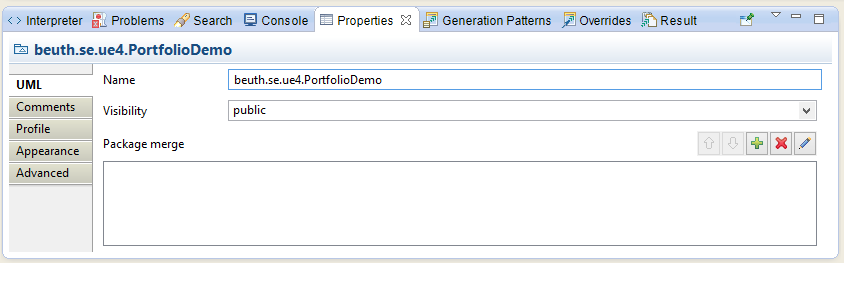
\includegraphics[width=0.8\textwidth]{./img/ProjectPackage.png}
\caption{Name des Modelles und gleichzeitig Hauptpaket des
GWT Projekts}\label{Fig:mainpackage}
\end{center}
\end{figure}

\newpage
\section{Klassenaufbau}
Die grundlegendsten Elemente in dem Modell sind \texttt{ViewImpl}-Klassen. Ein
Beispiel dafür ist in Abbildung \ref{Fig:viewimpl} zu sehen. Für jede dieser
Klassen Objekte werden mithilfe des Generators alle notwendigen Dateien
erzeugt, die für den späteren Seiteaufruf notwendig sind.

\begin{figure}[htbp]
\begin{center}
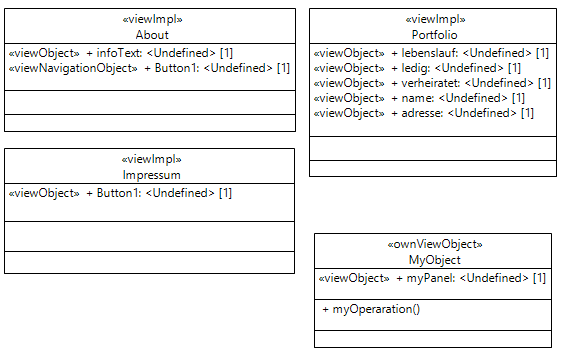
\includegraphics[width=1.0\textwidth]{./img/GWT-Model-Views-alg.png}
\caption{\texttt{ViewImpl}-Klassen zur Erzeugung von Seiten
für den Webauftritt.}\label{Fig:viewimpl}
\end{center}
\end{figure}

Des weiteren ist in der Abbildung \ref{Fig:viewimpl} ein Beispiel für ein
\textit{ownViewObject} zu sehen. Diese sind für komplexere oder mehrfach
verwendete UI-Struckturen gedacht und werden vom Generator als eigenständige
Klasse generiert.

GWT bietet, durch Verwendung des MVP Pattern, eine einfache Möglichkeit Seiten
auszutauschen. Um dieses Verfahren mit zu generieren wurde sich dazu
entschlossen, neben der Standardgenerierung von Seiten, eine zusätzliche
Methode einzubauen. Diese Methode bietet die Möglichkeit beliebig viele
alternativ Seiten für eine Ansicht im Webauftritt zu erzeugen (siehe Abbildung
\ref{Fig:viewInterface}). Die Möglichkeit der einfachen Austauschbarketi von
Views, wurde bei GWT unter anderem für Testzwecke angedacht.

\begin{figure}[htbp]
\begin{center}
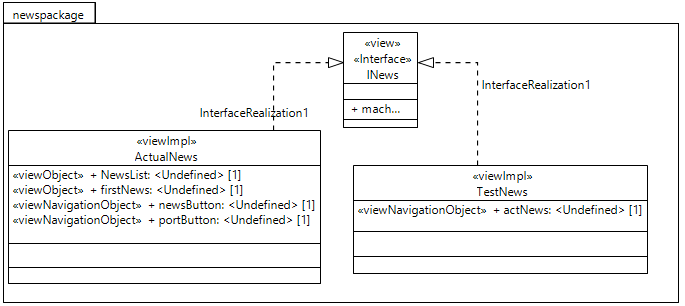
\includegraphics[width=1.0\textwidth]{./img/GWT-Model-Views-interface.png}
\caption{Ein Beispiel für die Verwendung der \texttt{ViewInterface}-Klassen
um mit Hilfe einer Vielzahl von \texttt{ViewImpl}-Klassen
eine austauschbare Ansicht zu erzeugen.}\label{Fig:viewInterface}
\end{center}
\end{figure} 

Bei dem, in Abbildung \ref{Fig:viewInterface}, gezeigtem M1 Modell Ausschnitt
wird die Komplette Klassenstruktur nicht zweimal erzeugt, anders als im
allgemeinem Fall (siehe Abbildung \ref{Fig:viewimpl}). Die
\texttt{'Name'Activity.java}, \texttt{'Name'Place.java} und \\
\texttt{'Name'View.java} Klassen werden hierbei nur einmal für das Interface
und die \texttt{'Name'ViewImpl.java} und \texttt{'Name'ViewImpl.ui.xml}
Dateien für jede realisierende \texttt{ViewImpl}-Klassen generiert. 

Darüber hinaus ist in Abbildung \ref{Fig:viewInterface} zu sehen, dass es
möglich ist, Klassen zu Paketen zuzuordnen. Auf diese Weise wird es
ermöglicht die zu generierenden Dateien zu gruppieren. 

\newpage
Das letzte in dem Modellen genutzte Klassenkonstrukt, sind die sogenannten
\texttt{PermanentView}-Elemente. Diese sind dazu gedacht, um zum Beispiel Menüs
zu erzeugen. Diese haben die Eigenschaft das sie auf allen Seiten zur Verfügung
stehen und nicht mehrfach generiert werden sollen.

\begin{figure}[htbp]
\begin{center}
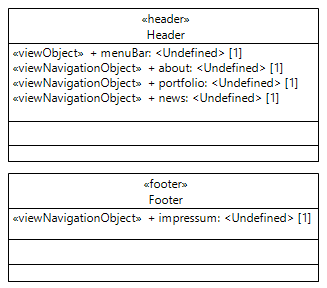
\includegraphics[width=0.55\textwidth]{./img/Header_Footer.png}
\caption{\texttt{PermanentView}-Elemente am Beispiel
eines Headers, mit Menu, und eines Footers.}\label{Fig:headerFooter}
\end{center}
\end{figure} 

\section{Seitenaufbau}
Je nach Art der Seite muss zuerst definiert werden, um was für einen Typ von
Seite es sich handelt. In Abbildung \ref{Fig:SideProp} ist ein Beispiel dafür
zu sehen, welches eine \textit{ViewImpl} und ein \textit{Header} zeigt, eine
spezialisierte Form der \textit{PermanentView}, zu sehen. Wichtig ist hier
die \texttt{concreteBinding}-Eigenschaft. An dieser Stelle kann bei Verwendung
eines separaten Interfaces festgelegt werden, welche konkrete implementierung
dargestellt werden soll, um keine Laufzeitfehler zu erzeugen muss zu jeder View
exakt eine ViewImpl angegeben werden. Diese Einstellung kann später im
Quellecode geändert werden.

\newpage
\begin{figure}[htbp]
\begin{center}
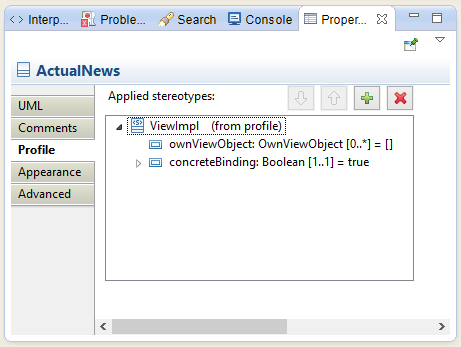
\includegraphics[width=0.8\textwidth]{./img/Prop-ViewImp.png}
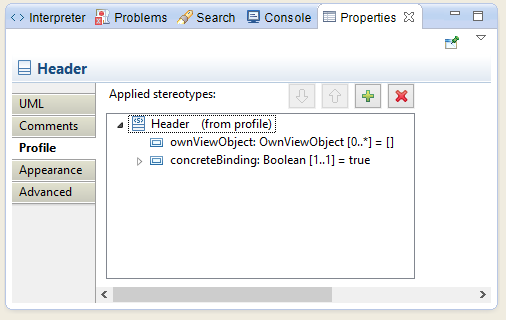
\includegraphics[width=0.8\textwidth]{./img/Prop-Header.png}
\caption{Klassen mit definierten Stereotypen, oben
eine \textit{ViewImpl} und unten ein \textit{Header}}\label{Fig:SideProp}
\end{center}
\end{figure} 

Um diese Seite mit Inhalten zu befüllen, können \textit{ViewObject}s und 
\textit{ViewNavigationObject}s als Attribute hinzugefügt werden.

\newpage
Bei \texttt{ViewObject}-Elementen können die in Abbildung \ref{Fig:ViewProp}
dargestellten Eigenschaften verändert werden.

\begin{figure}[htbp]
\begin{center}
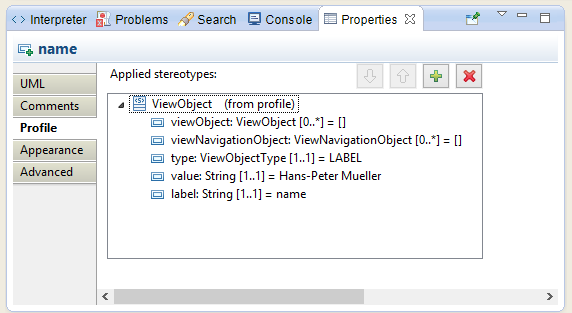
\includegraphics[width=0.8\textwidth]{./img/Prop-ViewObjects.png}
\caption{Eigenschaften eines \texttt{ViewObject}-Elementes }\label{Fig:ViewProp}
\end{center}
\end{figure} 

Bei \texttt{ViewNavigationObject}-Elementen können die in Abbildung
\ref{Fig:ViewNavProp} dargestellten Eigenschaften verändert werden. Hier ist
vor allem die letzte Eigenschaft \texttt{goToView} zu beachten, welche angibt
wohin dieses navigieren soll.

\begin{figure}[htbp]
\begin{center}
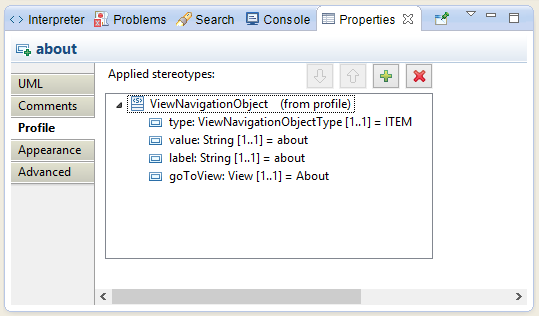
\includegraphics[width=0.8\textwidth]{./img/Prop-ViewNavigationObjects.png}
\caption{Eigenschaften eines \texttt{ViewNavigationObject}-Elementes
}\label{Fig:ViewNavProp}
\end{center}
\end{figure}

\chapter{Generator}
\label{Generator}
\chapter{Ergebnis} \label{Ergebnis}

Das Ziel bestand darin eine Grundarchitektur für ein GWT-Projekt zu erzeugen,
welche es dem Entwickler vereinfachen soll seine Anwendung gemäß dieser
Architektur zu erstellen.
Um das Projekt vollständig lauffähig zu machen, sind noch ein paar Handgriffe
vornehmen.

\begin{itemize}
  \item \texttt{AppEntryPoint.java} \\
  Hier muss defieniert werden, welche der Views die Start Seite werden soll.
  \item \texttt{AbstractView.java} \\
  In dieser Klasse ist es möglich eine Standard Größe für alle Seiten zu
  bestimmen.
  \item \texttt{ProductionGinModule.java} \\
  Auch hier muss wie in der AppEntryPoint-Klasse noch einmal die Start Seite
  definiert werden.
  \item \texttt{index.html und style.css} \\
  Diese beiden Dateien müssen nach dem Durchlauf des Generators in den 'war'
  Ordner verschoben werden. Sie dienen als Ausgangspunkt für die Webanwendung.
  \item \texttt{Zusätzliche Bibliotheken}\\
  	Zusätzlich zu den \texttt{GWT SDK} und \texttt{App Engine SDK} müssen die
    hier aufgeführten \texttt{.jar} Bibliotheken in das Projekt hinzugefügt
    werden.
  	\begin{itemize}
  	  \item \texttt{gin-2.0.jar}
  	  \item \texttt{guice-3.0-no\_aop.jar}
  	  \item \texttt{guice-assistedinject-3.0.jar}
  	  \item \texttt{gwt-servlet.jar}
  	  \item \texttt{javax.inject.jar}
	\end{itemize}
\end{itemize}
Zum Zeitpunkt der Entstehung dieser Arbeit ist es noch die folgenden
zwei Schritte notwendig.
\begin{itemize}
  \item \texttt{Imports} \\
  Es ist notwendig die noch fehlenden Imports in den Java-Klassen
  einzufügen, da diese aus Zeitgründen nicht vollständig eingearbeitet worden
  sind.
  \item \texttt{'Name'ViewImpl.ui.xml} \\
  In diesen Dateien müssen doppelte Elemente entfernt werden, die der Generator zu
  viel eingefügt hat, näheres dazu in Abschnitt \ref{Probleme}.
\end{itemize} 

Sind diese Änderungen vorgenommen, ist das Projekt lauffähig. Zusätzlich können
weitere Änderungen vorgenommen werden, zum Beispiel können weitere Texte eingefügt
oder das Design angepasst werden, dieses wurde von dem Generator nur rudimentär,
in Form einer \texttt{css}-Datei angelegt.

\section{Beispiel Anwendung}
Für das in diesem Abschnitt gezeigte Beispiel wurde das M1 Modell aus Abbildung
\ref{Fig:ergModell} verwendet. Zu sehen sind fünf Seiten, welche in Paketen
gegliedert sind. Darüber hinaus wurden zwei PermanentViews modelliert. Eine
Betrifft den Header, mit einem eingebautem Menu und eine den Footer, in dem
eine Navigation zum Impressum vorgesehen ist.

\begin{figure}[htbp]
\begin{center}
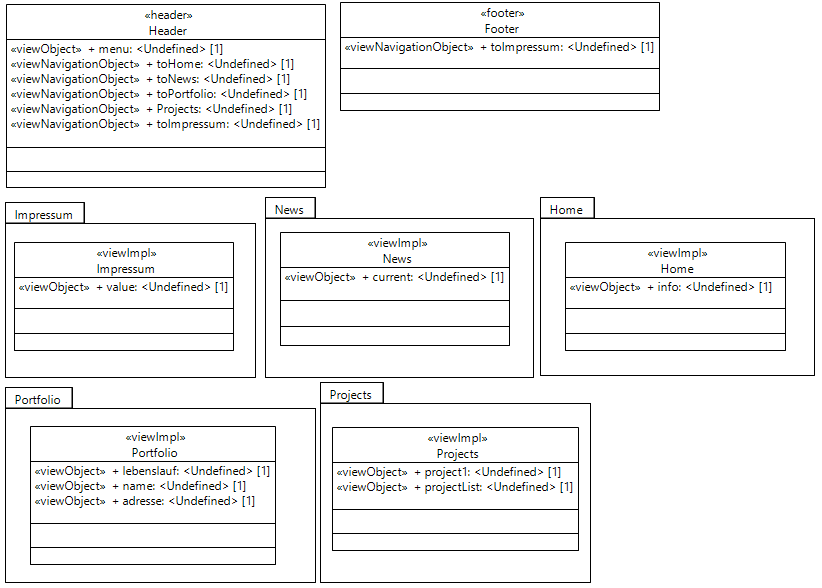
\includegraphics[width=0.8\textwidth]{./img/Model2.png}
\caption{Verwendetes Modell}\label{Fig:ergModell}
\end{center}
\end{figure}

Durch die extra eingebauten Pakete erweitert sich die Grundstruktur des
Projektes, in Abbildung \ref{Fig:packegeModel} ist auf der linken Seite die
komplette Packetstruktur des Projektes zu sehen. Hier ist zu erkennen, dass
für die fünf Seiten separate Pakete existieren. Jedoch für den Header und den
Footer keine zusätzlichen Pakete angelegt worden sind. Auf der rechten Seite in
Abbildung \ref{Fig:packegeModel}, wird der Inhalt einiger der Pakete näher
gezeigt. Hier ist zu erkennen, dass die beiden \texttt{ViewImpl}, die nicht in
Paketen liegen, direkt in dem \texttt{view} Paket liegen. Zusätzlich sind die
Klassen \texttt{Activity}, \texttt{Place}, \texttt{View} und die
\texttt{.ui.xml} Datei in dem Paket zu sehen. Am Beispiel der
\texttt{Home}-Seite ist gezeigt, dass die hierfür generierten Klassen und
Dateien in einem separaten Paket von \texttt{view}, nämlich in \texttt{home}
liegen.

\begin{figure}[htbp]
\begin{center}
\raisebox{3.2cm}{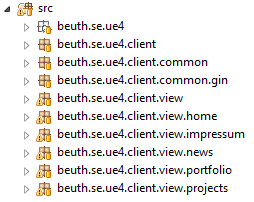
\includegraphics[width=0.4\textwidth]{./img/Packages.png}}
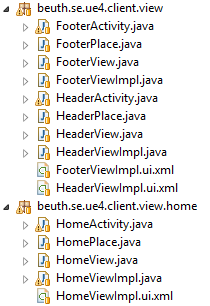
\includegraphics[width=0.4\textwidth]{./img/PackagesExample.png}
\caption{Generierte Paketstruktur, links gesamte
Paketstruktur im Überblick; rechts Beispiel für das
Strukturieren im Modell, mit zusätzlichen Paketen}\label{Fig:packegeModel}
\end{center}
\end{figure}
 
In diesem Beispiel soll die \texttt{home} Seite die Startseite für die
Webanwendung darstellen. Aus diesem Grund wurde entsprechend in der
\texttt{AppEntryPoint}- und der \texttt{ProductionGinModule}-Klasse die
jeweilige Klasse für die StartView angegeben. (Listing \ref{lst:appEntryPoint}
und \ref{lst:ProductionGinModule}) 
\lstset{language=gwt}
\begin{lstlisting}[caption={Änderung an der \texttt{AppEntryPoint}-Klasse zur
Bestimmung der Startseite}, label={lst:appEntryPoint}] 
[..]
  historyHandler.register(injector.getPlaceController(), eventBus,
      new HomePlace());
[..]
\end{lstlisting}
\lstset{language=gwt}
\begin{lstlisting}[caption={Änderung an der \texttt{ProductionGinModule}-Klasse
zur Bestimmung der Startseite}, label={lst:ProductionGinModule}] 
[..]
  bind(HomeView.class);
[..]
\end{lstlisting}

Zusätzlich wurde an einigen Stellen der Inhalt der Seiten erweitert. Dies ist
einerseits dadurch möglich, dass innerhalb der \texttt{ViewImpl} Klasse
zusätzlicher Inhalt eingefügt werden kann (Listing \ref{lst:conntentJava}), aber
anderseits innerhalb der \texttt{.ui.xml}-Datei (Listing \ref{lst:conntentUI}).

\lstset{language=gwt}
\begin{lstlisting}[caption={Einfügen von Inhalten auf einer Seite durch
Veränderungen am Java-Code},
label={lst:conntentJava}] 
[..] 
  HTML html = new HTML("<div><h1>Brandhei&szlig;e News</h1>"
	+"Lorem ipsum [..] amet."
	+"<div/>");
  content.add(html);
[..]
\end{lstlisting}
\lstset{language=gwt}
\begin{lstlisting}[caption={Einfügen von Inhalten auf einer Seite durch
Veränderungen am \texttt{ui.xml}-Datei},
label={lst:conntentUI}] 
[..] 
 <g:FlowPanel>
	<!-- InteractionElements -->
	<!-- Start of user code Home 
	     Start protectetRegion -->
			<g:Label text=" Lorem [..] facilisi. "/>
			[..]		
	<!-- End of user code -->
	</g:FlowPanel>
[..]
\end{lstlisting}

Dieses sind nur zwei Arten wie die Anwendung weiter bearbeitet werden kann,
nachdem der Quellecode aus dem M1 Modell generiert worden ist. Zum Einen
unterstützen der Generator und das Profil derzeit nicht alle von GWT
bereitgestellten UI Elemente, sodass diese nachträglich eingefügt werden
müssen. Da diverse UI Editoren existieren, welche das Erzeugen einer
Benutzeroberfläche grafisch unterstützen, wurde sich in dieser Arbeit bewusst
gegen das Erzeugen einer Webanwendung, die vollständig designt worden ist,
entschieden. 

\chapter{Fazit und Ausblick}
\label{FazitAusblick}
Anhand des Ergebnisses wird deutlich, dass mit dem Generator Projekt und einigen
kleineren Änderungen im generiertem Code eine funktionierende GWT Frontend
Anwendung erzeugt werden kann. Durch einen
hohen Abstraktionsgrad innerhalb des UML-Profils wird die Entwicklung einer solchen Anwendung 
vereinfacht und die Fehleranfälligkeit auf ein geringes Maß minimiert ohne
Einschränkungen bei der vorgegebenen Zielarchitektur (vgl. Abschnitt
\ref{AufBZielArchitektur}).
Darüber hinaus sind die durch GWT und MVP gegebenen Vorteile z.B. der
einfache Austausch von Views weiterhin und teilweise leichter nutzbar z.B.
durch Aus- und Einkommentierung bei dem Austausch von Views. Zur Gestaltung der
Website stehen einem Entwickler alle Möglichkeiten z.B. die
Nutzung von Ui-Editoren weiterhin ohne Einschränkungen zur Verfügung und die
Anwnendungsfälle sind frei wählbar, wie anhand der 2 M1-Modelle deutlich wird.
Es können eigene View Elemente erstellt und eingebunden werden, welches die
Architekturkonzepte zusätzlich unterstützt. Des weiteren wird die Navigation
über ViewNavigationObjects innerhalb der Seiten generiert, jedoch ist weiteres
Verhalten wie z.B. das Öffnen eines Popups nicht umgesetzt.

Durch Abschnitt \ldots ref wird ersichtlich, dass die vorzunehmende Änderung im
Bereich der View Komponenten innerhalb der ui.xml Datei keine optimale Lösung ist. Dies wird hervorgerufen
dadurch, dass ViewObjects weitere ViewObjects beinhalten können und somit in der
ui.xml mehrfach enthalten sein können. Dies führt zu dem Gedanken, dass eine
andere Generierungssprache außerhalb von OCL potenziell besser geeignet wäre, da
keine weitere Möglichkeit gefunden werden konnte einen optimalen Lösungsansatz
umzusetzen u.A. durch das verändern einer Variable innerhalb einer if-Bedingung.
Eine weitere Möglichkeit der Optimierung an dieser Stelle könnte darin bestehen,
dass Backend generierbar zu machen. Dadurch können Datenmodelle zu dem
UML-Profil hinzugefügt werden, welche auch die Grundlage für View Komponenten
bilden können. Anhand eines
Beispiels kann das Datenmodell einer Produktklasse mit den Attributen Name,
Preis und Verkaufsort dazu genutzt werden, dass innerhalb einer View automatisch
eine Tabelle generiert wird, welche als Spalten die Attribute beinhaltet und
alle Produkte anzeigt. Dieser Lösungsansatz wäre einerseits eine
Weiterentwicklung des Generatorprojekten bietet jedoch noch keine Komplettlösung, sollten Views auch
ohne Datenmodelle generiebar sein.

Weiterhin müssen strukturelle Änderungen z.B. das Umsetzen der
index.html oder das Hinzufügen von Bibliotheken z.B. GIN (vgl. Abschnitt ref
\ldots) innerhalb des GWT Projektes vorgenommen werden. Diese Änderungen können
durch die Verbindung des Generator Projektes mit Maven vermieden werden.

Das zu generierende M1-Modell weist keine Assoziationen auf, wodurch viele
Eigenschaften wie das Beinhalten von eigenen View Objekten in Views versteckt
bleiben. Aus diesem Grund wäre eine Generierung eines UML Klassendiagramms als
Weiterentwicklung ein wichtiger aspekt. Dadurch wird zusätzlich der im Fokus
liegende architektonische Aspekt des Generator Projektes hervorhebt. Darüber
hinaus sind viele Teile wie z.B. die einmalig vorhandenen Klassen sowie die View
Klassen z.B. Activity, Place und ViewImpl.ui.xml in dem M1-Modell nicht
ersichtlich bzw. nicht vorhanden, wodurch das generierte unübersichtlich werden
kann. Weshalb ein UML Klassendiagramm weiterhin stark unterstützend wirkt. 

Eine weitere Möglichkeit Übersicht zu schaffen besteht zusätzlich darin
Activitätsdiagramme zu generieren. Dies ermöglicht einen weiteren Überblick über
die generierte Navigation.

Zusammenfassend ist zu erwähnen, dass das Generatorprojekt eine gute
Grundlage für die Weiterentwicklung darstellt unter der Vorrausetzung, dass die
Redundanz und Strukturierung des Generators verbessert wird.
\chapter{Arbeitsaufteilung}
\label{Arbeitsaufteilung}
In diesem Projekt wurde der schriftliche Teil klar getrennt.

Stephanie hat die Kapitel MDA, UML Profil auf M2 Ebene und Generator
geschrieben.
Marcus hat die Kapitel Dependency Injection, Aufbau und Struktur M1 Modell und
das Ergebnis gechrieben.
Claudia hat die Kapitel GWT, Konzeption und Fazit und Ausblick geschrieben.

Dagegen wurde der praktische Teil und die Konzeption des Projektes nicht
strikt aufgeteilt. In den meisten Fällen waren alle gemeinsam an dem Projekt
beteiligt.

Wir würden uns jedoch gerne nach der Notenbekanntgabe die Möglichkeit offen
halten, die Noten innerhalb des Teams evtl. umverteilen zu dürfen.


%----------------------------------------------------------------------------------------
%	BIBLIOGRAPHY
%----------------------------------------------------------------------------------------
\label{Literaturverzeichnis}
\bibliographystyle{apalike}
\bibliography{bib}
\end{document}
